\chapter{High Energy QCD}
\label{chap:HEQCD}

	{\color{red}
	Stuff for this section
	\begin{itemize}
		\item \st{s, t, u gives log mini-calc,}
		\item HE limit of gg-> gg gives log (at LO),
		\item Tiny bit about cuts S matrix to Optical theorem,
		\item NLO calculation of leading part of gg->gg (explain sub-leading bits) - do this bit using cuts,
		\item Extra real corrections and writing these as contractions of currents,
		\item A bit on HE phase-space integrals?
	\end{itemize}
	}

	In this chapter we look in detail at the `High Energy' limit of QCD.  We begin by defining this limit and
	looking at how basic $2\rightarrow2$ scattering behaves at leading order and next-to-leading order in
	$\alpha_s$.

	\section{The `High Energy' limit}
		\label{sub:HElimit}

		The `High Energy' limit of QCD, also referred to as the Multi-Regge Kinematic (MRK) limit is
		defined in terms of the kinematics of the final state.  We require a \emph{strong rapidity ordering}
		of all outgoing radiation as well as all the emissions having \emph{similar transverse momenta}.
		Mathematically this is:

		\begin{equation}
			y_1\gg y_2\gg\cdots\gg\\y_n \text{ and } |p_{\perp1}| \approx |p_{\perp2}| \approx\cdots\approx|p_{\perp(n-1)}|,
			\label{eqn:MRK}
		\end{equation}

  		where we define the rapidity of a final states particle as

		\begin{equation}
			y = \half\frac{E+p_z}{E-p_z}
			\label{eqn:rap}
		\end{equation}

		where $E$ is the energy of particle and $p_z$ it the $z$ component of its momentum. We can
		state the of the criteria in eq. \eqref{eqn:MRK} equivalently as $s_{ij}\rightarrow\infty$ where
		$s_{ij} = (p_i + p_j)^2$.  We sometimes instead use the pseudo-rapidity, $\eta$, which is
		simply related to the angle of the outgoing state to the beam, $\theta$:

		\begin{equation}
			\eta = -\ln\tan\frac{\theta}{2}.
			\label{eqn:prap}
		\end{equation}

		For massless states eqs. \eqref{eqn:rap} and \eqref{eqn:prap} are equivalent.

	\section{Mandelstam Variables in the High Energy Limit}
		\label{sub:MandelstamVariables}

		The $2\rightarrow 2$ QCD scattering amplitudes can be expressed in terms of the well-known Mandestam
		variables $s$, $t$ and $u$.  Which, in terms of the momenta in the process, are given by:

		\begin{subequations}
			\begin{equation}
				s = (p_1 + p_2)^2
			\end{equation}
			\begin{equation}
				t = (p_1 - p_2)^2
			\end{equation}
			\begin{equation}
				u = (p_2 - p_3)^3
			\end{equation}
			\label{eqn:mandel}
		\end{subequations}

		When working in the high energy limit it is convenient to re-express these in terms of the
		perpendicular momentum of the outgoing partons, $p_\perp$, and the difference in rapidity
		between the two final state partons, $\Delta y$.  If we parametrise our outgoing states as

		\begin{align}
		\begin{split}
			p_1 = p_{\perp1}(\cosh y_1, \cos\phi_1, \sin\phi_1, \sinh y_1),\\
			p_2 = p_{\perp2}(\cosh y_2, \cos\phi_2, \sin\phi_2, \sinh y_2),
		\end{split}
		\end{align}

		then we can express eqs. \eqref{eqn:mandel} as follows

		\begin{subequations}
			\begin{equation}
				s = 4p_\perp^2 \cosh^2\frac{\Delta y}{2},
			\end{equation}
			\begin{equation}
				t = -2p_\perp^2 \cosh\frac{\Delta y}{2}e^{-\frac{\Delta y}{2}},
			\end{equation}
			\begin{equation}
				u = -2p_\perp^2 \cosh\frac{\Delta y}{2}e^{\frac{\Delta y}{2}}.
			\end{equation}
		\end{subequations}

		In the limit of hard jets well separated in rapidity, i.e. $\Delta y\rightarrow\infty$,
		these are well approximated by

		\begin{subequations}
			\begin{equation}
				s = p_\perp^2 e^{\Delta y}
			\end{equation}
			\begin{equation}
				t = -p_\perp^2
			\end{equation}
			\begin{equation}
				u = -p_\perp^2 e^{\Delta y}
			\end{equation}
		\end{subequations}

		From this it is clear that the `hard, wide-angle jet' limit is equivalent to the High Energy
		limit since as $\Delta y$ grows large $s$ will grow exponentially while $t$ will stay fixed.
		Rearranging for $\Delta y$ in the above equations yields:

		\begin{equation}
			\Delta y = \ln \left(\frac{s}{-t}\right).
			\label{eqn:largeLogs}
		\end{equation}

		This is a useful result because it relates the simple kinematics of an event to a (potentially)
		large logarithm.  It is already naively clear from eq. \eqref{eqn:largeLogs} that a final state
		with large rapidity gaps could require a more careful inspection than the fixed-order approach
		discussed in section \ref{sec:pqcdAndResum}.

	\section{$qQ$-scattering at High Energy}

		Here we begin with the simplest example; the case of $qQ\rightarrow qQ$ for all negative helicity partons
		\footnote{where the capital $Q$ implies it is a different flavour to $q$ - and hence we need not consider the crossed
		diagrams which would contribute if they were the same flavour}. There is only one diagram which contributes shown
		in fig. (\ref{fig:TwoToTwo}).  Using the Feynman rules detailed in section \ref{sec:partonicCrossSection} we can
		write the matrix element as:

		\begin{align}
			i\mathcal{M}_{q^-Q^-\rightarrow q^-Q^-} &= ig_s^2T^d_{1a}T^d_{2b}\frac{\overline{u}^-(p_1)\gamma^\mu
			  u^-(p_a)\overline{u}^-(p_2)\gamma_\mu u^-(p_b)}{t}\\
			  &= ig_s^2T^d_{1a}T^d_{2b}\frac{\bk{1}{\mu}{a}\cdot\bk{2}{\mu}{b}}{t},
		\end{align}

		where $t = (p_a - p_1)^2$ and we have used the shorthand $\overline{u}^-(p_i)\gamma^\mu u^-(p_j) = \bk{i}{\mu}{j}$ in the second line.
		Writing the contraction of these two `current' terms in terms of light-cone coordinates we have:

		\begin{equation}
			i\mathcal{M}_{q^-Q^-\rightarrow q^-Q^-} = ig_s^2T^d_{1a}T^d_{2b}\frac{2\sqrt{p_a^-p_b^+}}{t}
			\left(\sqrt{p_1^+p_2^-}e^{i\phi_2} + \sqrt{p_1^-p_2^+}e^{i\phi_1}\right),
			\label{eqn:qQ2qQ}
		\end{equation}

		where $e^{i\phi_i} = \frac{p_{\perp i}}{|p_{\perp i}|}$.  We now approximate the kinematics in such a way that we may write
		eq. \eqref{eqn:qQ2qQ} in a `factorised' form once again.  Specifically we consider that the scattering can be thought
		of as two partons glancing off one another.  That is, we assume that $p_1^+\ll p_1^-$ and $p_2^-\ll p_2^+$.  We can further
		assume that $p_1^-\approx p_a^-$ and $p_2^-\approx p_b^-$ and with this we see that \eqref{eqn:qQ2qQ} becomes:

		\begin{equation}
			i\mathcal{M}_{q^-Q^-\rightarrow q^-Q^-} = \frac{2s}{t}\left(g_sT^d_{1a}e^{i\phi_1}\right)\left(-ig_sT^d_{2b}\right),
			\label{eqn:reggeTraj}
		\end{equation}

		which is `factorised' in the sense that each scalar term in brackets depends only on one quark line; either on the $p_{a/1}$
		line or the $p_{b/2}$ line.  We see that the amplitude for $qQ\rightarrow qQ$ is dominated by the $s$ kinematic variable.
		We can express this as:

		\begin{equation}
			\mathcal{M}_{q^-Q^-\rightarrow q^-Q^-} \sim s^{\alpha(t)},
		\end{equation}

		which is exactly the behaviour expected when a particle exchanged in the $t$-channel has `reggeised
		\cite{sabioThesis,DelDuca:1995hf,lipatovBook}.  $\alpha(t)$ is the Regge trajectory and is equal to
		the intrinsic spin of the state exchanged.  In our example we have have a spin-one gluon exchanged
		and accordingly we can see from eq. \eqref{eqn:reggeTraj} that $\alpha(t)=2$ for $qQ\rightarrow qQ$.

		\begin{figure}
			\begin{center}
			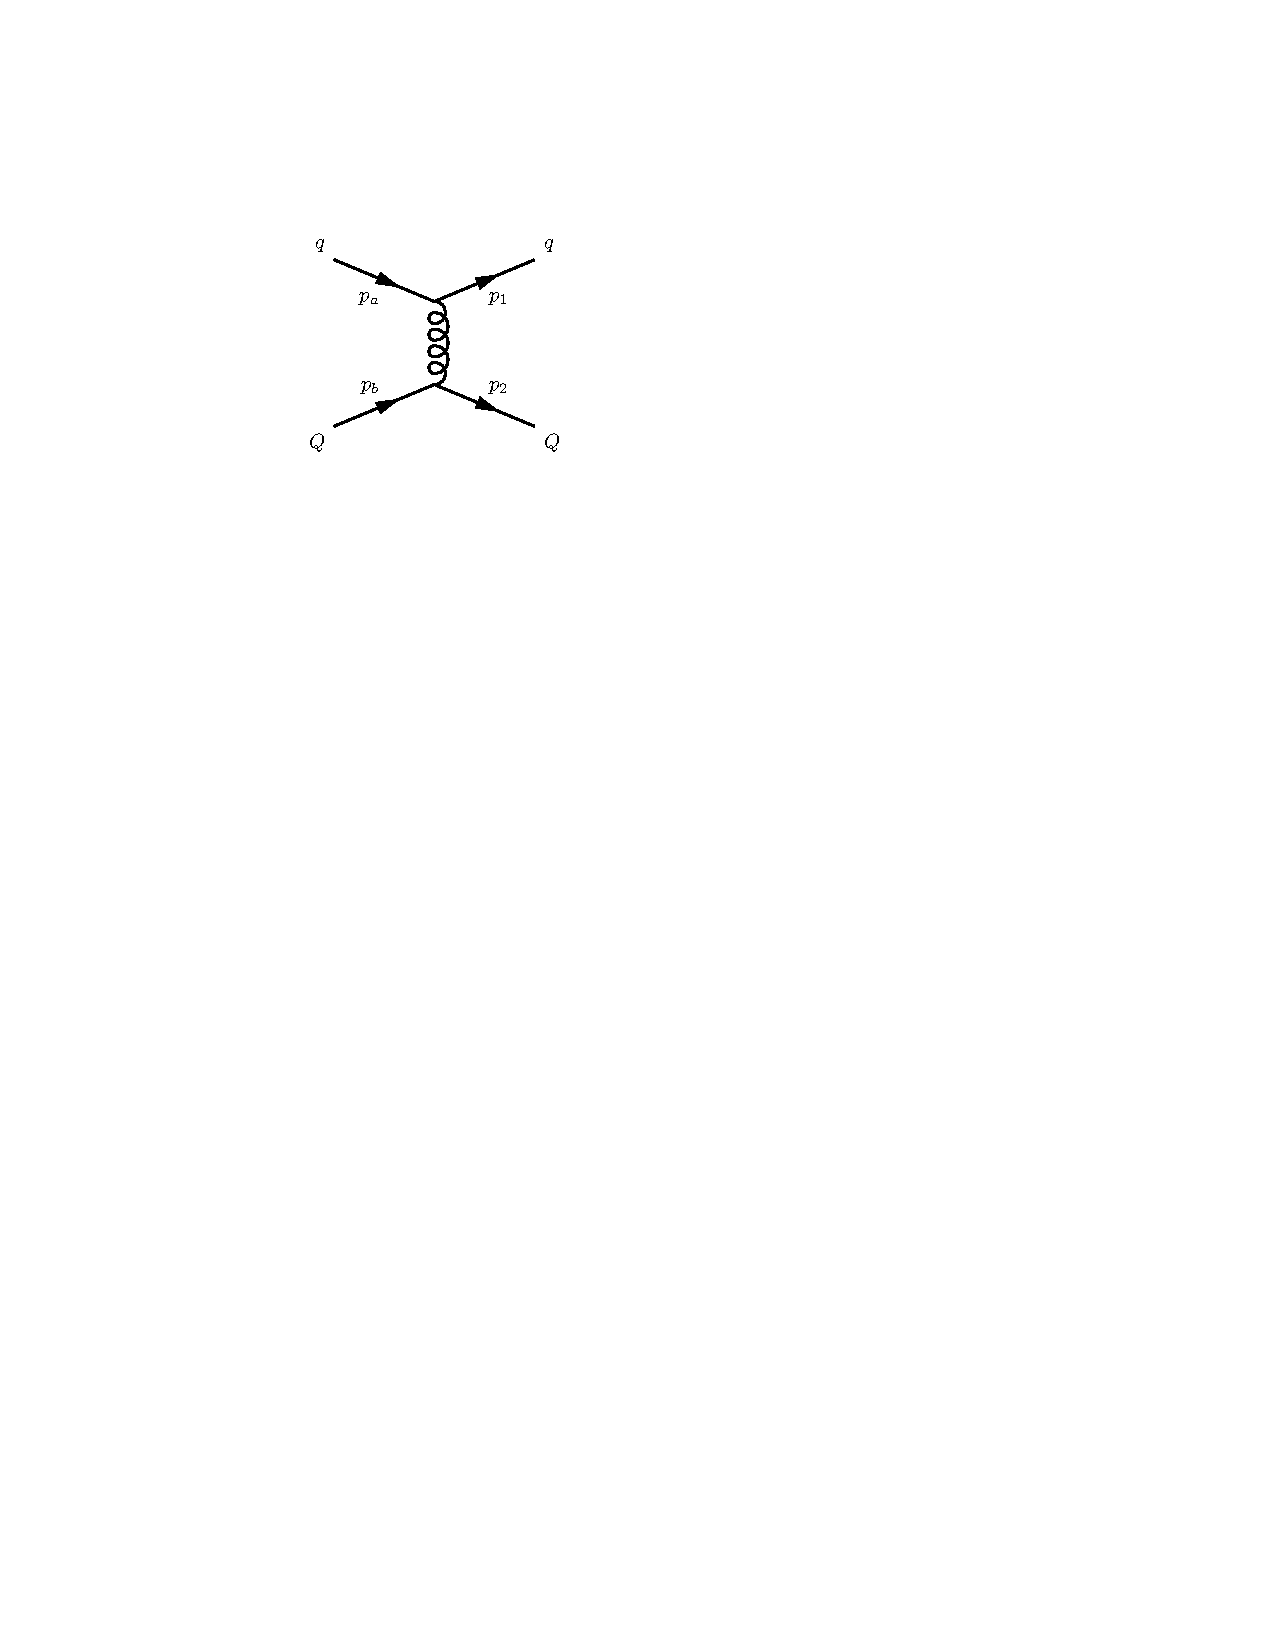
\includegraphics[width=0.35\linewidth]{TwoToTwo}
			\caption{The only diagram which contributes to $qQ\rightarrow qQ$ at leading order in $\alpha_s$.}
			\label{fig:TwoToTwo}
			\end{center}
		\end{figure}

	\section{$qg$ scattering at High Energy}

		We now with explore the more involved case of $2\rightarrow 2$ quark-gluon scattering.  At leading order this
		consists of three diagrams shown in fig. (\ref{fig:TwoToTwo}).  Here we only show the calculations
		for the helicity structure where both quark lines have fixed, and opposite, helicities.  We use
		the following gauge choice for the gluon polarisations:

		\begin{align}
		\epsilon^{+*}_{2\sigma}&=\frac{\langle b|\sigma|2\rangle}{\sqrt{2}\langle b2\rangle} & \epsilon^{-*}_{2\sigma} &= -\frac{\langle b|\sigma|2\rangle}{\sqrt{2}[b2]} \\
		\epsilon^{+}_{b\sigma}&=-\frac{\langle b|\sigma|2\rangle}{\sqrt{2}[2b]} & \epsilon^{-*}_{2\sigma} &= -\frac{\langle b|\sigma|2\rangle}{\sqrt{2}\langle 2b\rangle}
		\end{align}

		For simplicity we alter the notation slightly and choose to model everything as having negative helicity.
		To describe positive helicities we can use the transpose property shown in equation 16.

		\begin{figure}[h]
			\centering
			\begin{subfigure}[b]{0.3\textwidth}
				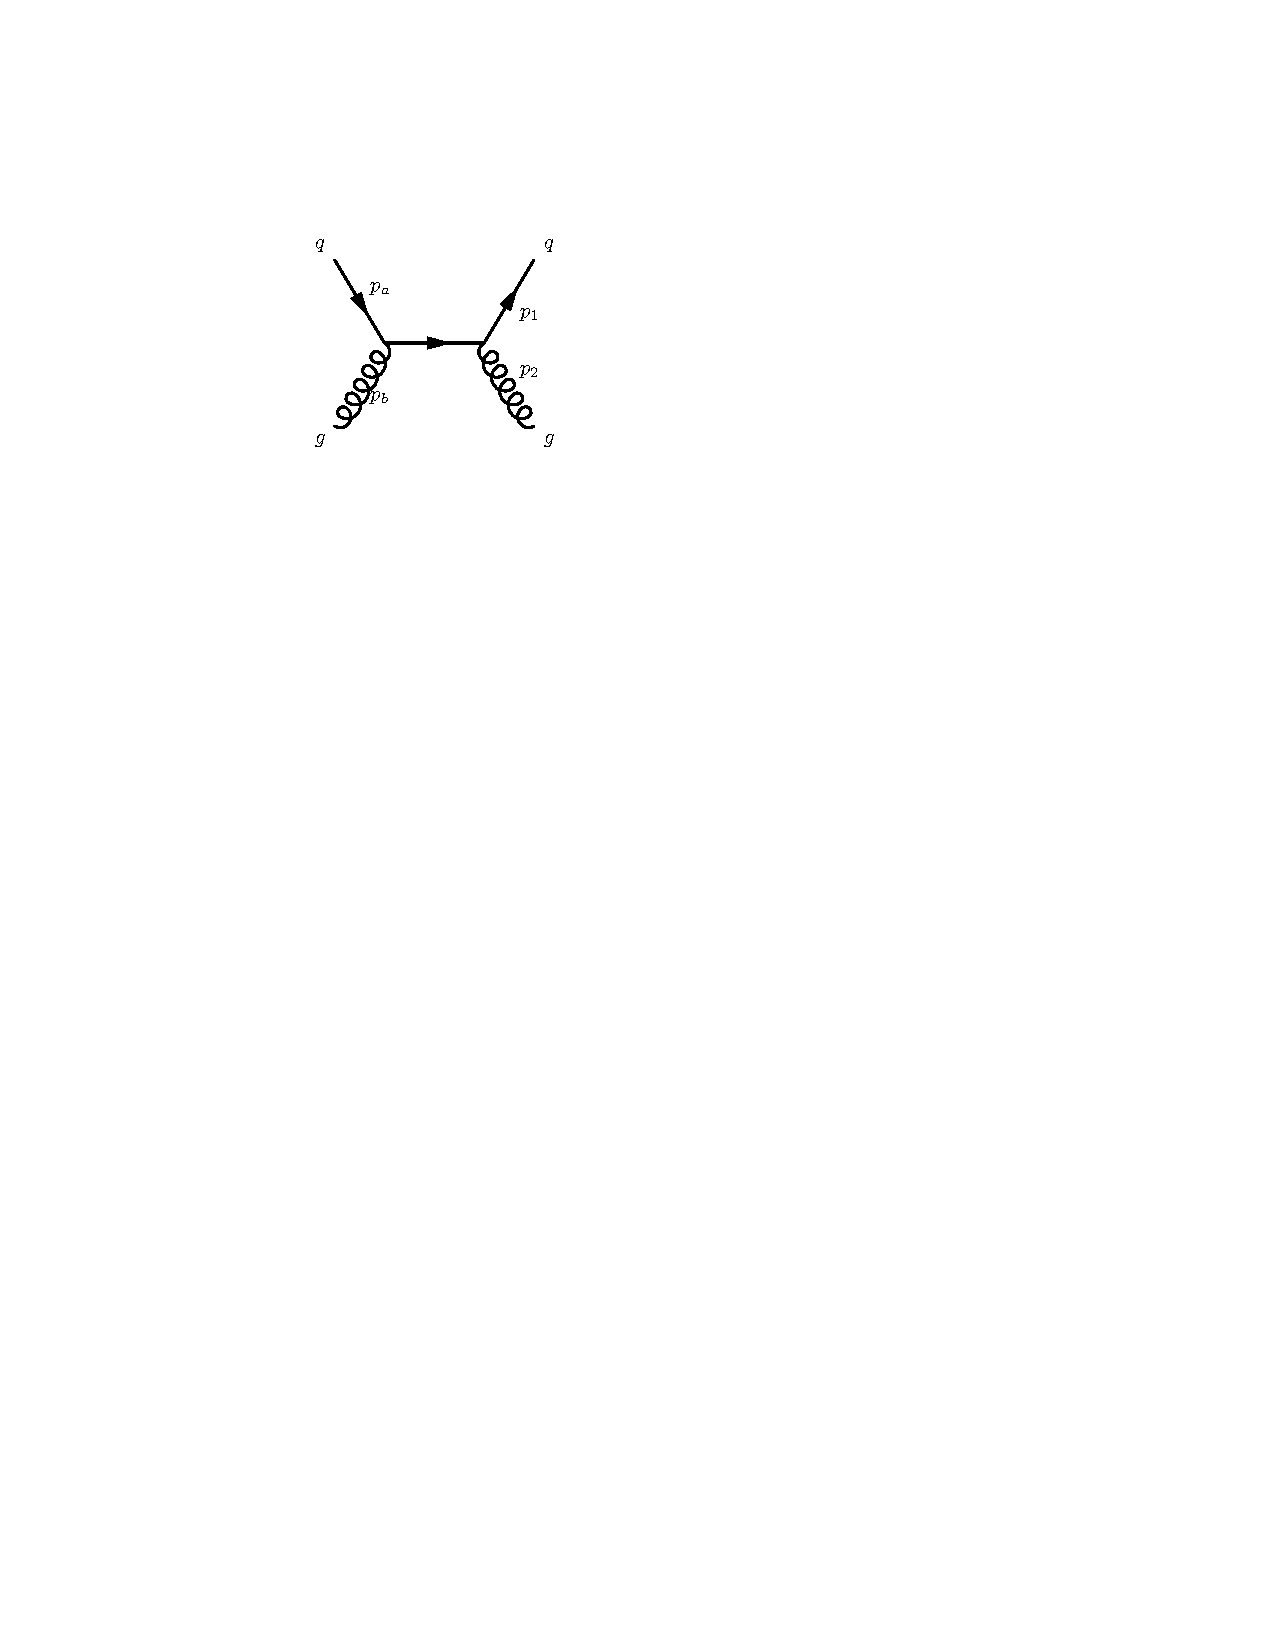
\includegraphics[width=\textwidth]{qg2qg-s}
				\caption{}
				\label{fig:qg2qg-s}
			\end{subfigure}

			\begin{subfigure}[b]{0.3\textwidth}
				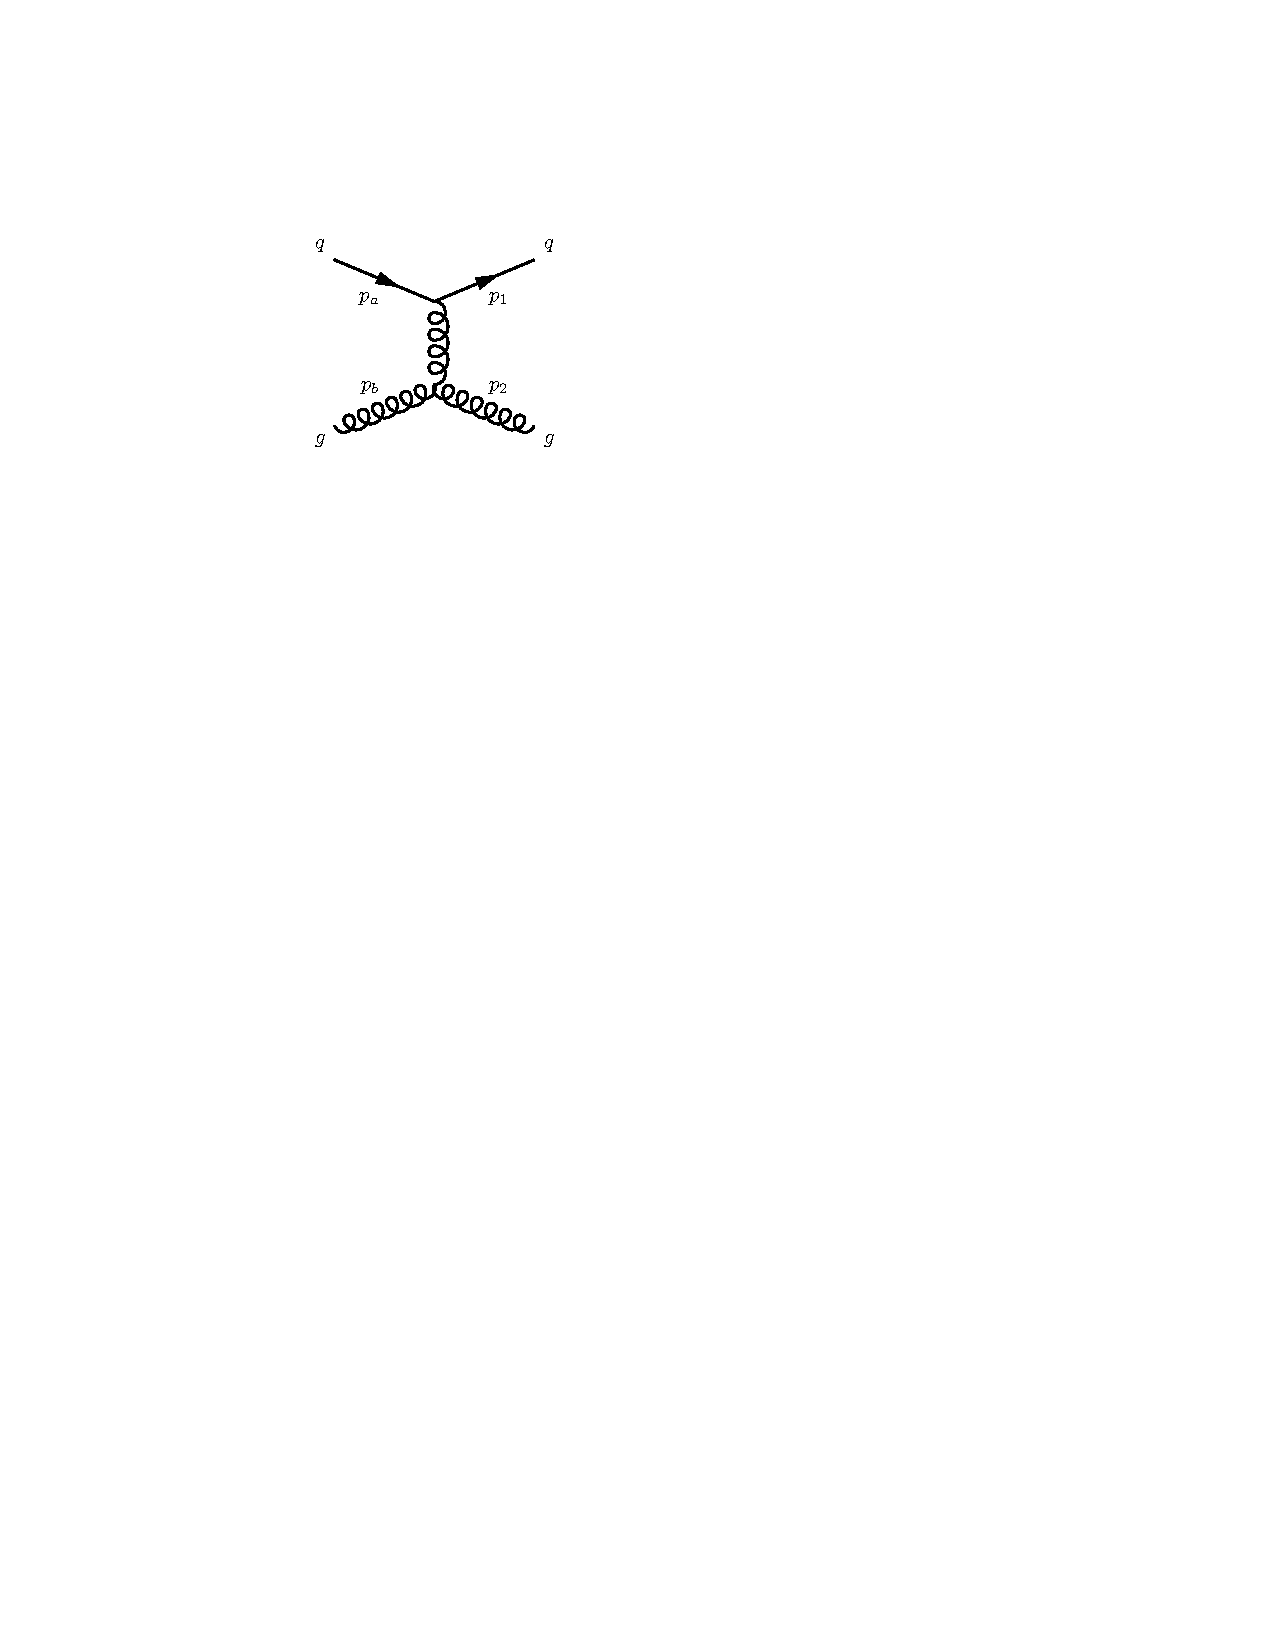
\includegraphics[width=\textwidth]{qg2qg-t}
				\caption{}
				\label{fig:qg2qg-t}
			\end{subfigure}
			~
			\begin{subfigure}[b]{0.3\textwidth}
				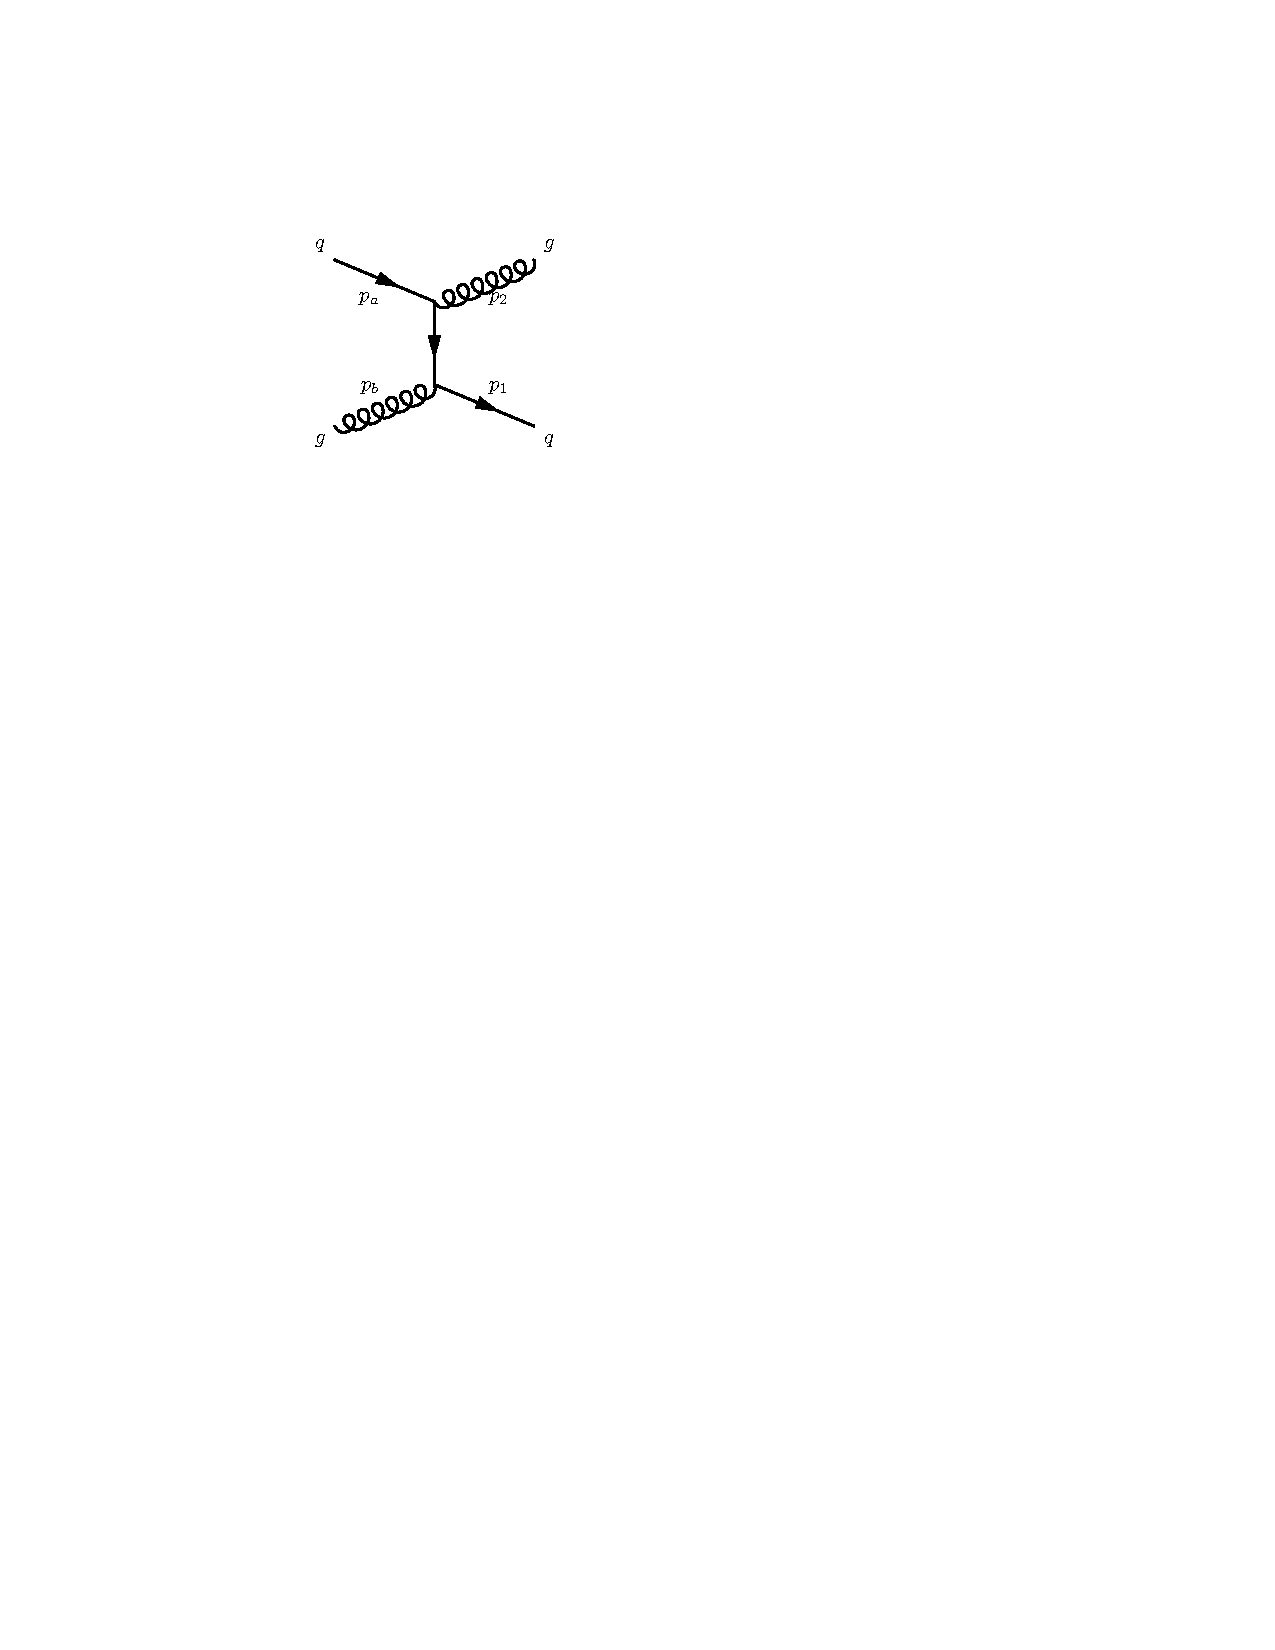
\includegraphics[width=\textwidth]{qg2qg-u}
				\caption{}
				\label{fig:qg2qg-u}
			\end{subfigure}
			\caption{The $s$, $t$ and $u$ channel diagrams contributing to $qg\rightarrow qg$ at leading
			         order in $\alpha_s$ in figures (\ref{fig:qg2qg-s}), (\ref{fig:qg2qg-t}) and (\ref{fig:qg2qg-u})
			         respectively.}
		\end{figure}

		\subsection{$s$-channel}

			The matrix element for the $s$-diagram is:

			\begin{equation}
			-_a-i\mathcal{A}_s=\overline{u}^-(p_1)\left(-\frac{ig_s}{2}\gamma^\mu\right)\epsilon_\mu^{*+}(p_2)
				\frac{i(\slashed q+mc)}{q^2-m^2c^2}\left(-\frac{ig_s}{2}\gamma^\nu\right)\epsilon^+_\nu(p_b)u^-(p_a),
			\end{equation}
			\begin{equation*}
				\Rightarrow \mathcal{A}_s=-\frac{g^2_s}{4q^2}\epsilon^{*+}_{2\mu}\epsilon^+_{b\nu}\overline{u}^-_1\gamma^\mu\slashed q\gamma^\nu u^-_a,
			\end{equation*}

			where we have used $q\gg mc$ for the high energy case.  The propagator has momentum $q=p_a+p_b=p_1+p_2$ therefore:

			\begin{equation}
				\mathcal{A}_s=-\frac{g^2_s}{4q^2}\frac{\langle{b}|\mu|2\rangle}{\sqrt{2}\langle{b2\rangle}}
				\frac{\langle{b}|\nu|2\rangle}{\sqrt{2}[2b]}\overline{u}^-_1\gamma^\mu(\slashed{p}_a+\slashed{p}_b)\gamma^\nu u^-_a,
				\end{equation}
			\begin{equation*}
				\Rightarrow\mathcal{A}_s=-\frac{g^2_s}{8q^2s_{2b}}\langle{b}|\mu|2\rangle\langle{b}|\nu|2\rangle
				\left(\overline{u}^-_1\gamma^\mu\gamma^\sigma\gamma^\nu u^-_ap_{a\sigma}+
				\overline{u}^-_1\gamma^\mu\gamma^\sigma\gamma^\nu u^-_ap_{b\sigma}\right),
			\end{equation*}

			where we have used equation 8.  The gamma matrices satisfy the Clifford algebra, $\{\gamma^\mu, \gamma^\nu\}=2g^{\mu\nu}$ and so we may write:

			\begin{equation}
				\overline{u}^-_1\gamma^\mu\gamma^\sigma\gamma^\nu u^-_ap_{a\sigma}=
				\overline{u}^-_1\gamma^\mu\gamma^\nu\gamma^\sigma u^-_ap_{a\sigma} -
				2\overline{u}^-_1\gamma^\mu g^{\sigma\nu}u^-_ap_{a\sigma}
			\end{equation}

			But in the MRK limit the Dirac equation is $\slashed{p}_au^-_a=0$:

			\begin{equation}
				\mathcal{A}_s=-\frac{g^2_s}{8q^2s_{2b}}\langle{b}|\mu|2\rangle\langle{b}|\nu|2\rangle
				\left(-2\overline{u}^-_1\gamma^\mu u^-_ap_{a}^\sigma+\overline{u}^-_1\gamma^\mu\gamma^\sigma\gamma^\nu u^-_ap_{b\sigma}\right)
			\end{equation}

			For the second term we must use the following identity:

			\begin{equation}
				\gamma^\mu\gamma^\sigma\gamma^\mu=g^{\mu\sigma}\gamma^\nu + g^{\sigma\nu}\gamma^\mu
				- g^{\mu\nu}\gamma^\sigma - i\epsilon^{\rho\mu\sigma\nu}\gamma_\rho\gamma^5,
			\end{equation}

			where $\epsilon^{\rho\mu\sigma\nu}$ is the $4D$ totally antisymmetric symbol:

			\begin{equation}
				\mathcal{A}_s=-\frac{g^2_s}{8q^2s_{2b}}\langle{b}|\mu|2\rangle\langle{b}|\nu|2\rangle
				\left(\langle 1|\mu|a\rangle p_a^\nu + p_{b\sigma}\overline{u}^-_1(g^{\mu\sigma}\gamma^\nu +
				g^{\sigma\nu}\gamma^\mu - g^{\mu\nu}\gamma^\sigma - i\epsilon^{\rho\mu\sigma\nu}\gamma_\rho\gamma^5)\right)
				\end{equation}
				\begin{equation}
				\Rightarrow\mathcal{A}_s=-\frac{g^2_s}{8q^2s_{2b}}\langle{b}|\mu|2\rangle\langle{b}|\nu|2\rangle
				\left(\langle 1|\mu|a\rangle \langle a|\nu|a\rangle\!+\!\langle b|\mu|b\rangle
				\langle 1|\nu|a\rangle\!+\!\langle b|\sigma|b\rangle\langle1|\sigma|a\rangle
				g^{\mu\nu}\!-\!i\langle b|\sigma|b\rangle\langle 1|\epsilon^{\rho\mu\sigma\nu}\gamma_\rho\gamma^5|a\rangle\right)
			\end{equation}

			The second, third and fourth terms are zero because, for example:

			\begin{equation}
				\langle b|\mu|2\rangle\langle b|\mu|b\rangle = 2[2b]\langle b b\rangle = 0
			\end{equation}

			\begin{equation}
				\Rightarrow\mathcal{A}_s=-\frac{g^2_s}{8q^2s_{2b}}
				\langle{b}|\mu|2\rangle\langle{b}|\nu|2\rangle\langle{1}|\mu|a\rangle\langle{a}|\nu|a\rangle
			\end{equation}

			Where we have used equation 10.

			\begin{equation}
			\mathcal{A}_s=-\frac{g^2_s}{4q^2s_{2b}}[2a]\langle ab\rangle\langle{b}|\mu|2\rangle\langle{1}|\mu|a\rangle
			\end{equation}

			And using $q^2=s_{ab}=\langle ab\rangle[ba]$ and $s_{2b}=\langle2b\rangle[b2]$ we have:

			\begin{equation}
			\mathcal{A}_s=-\frac{g^2_s}{4}\frac{[2a]\langle ab\rangle}{\langle ab\rangle[ba]
			\langle2b\rangle[b2]}\langle{b}|\mu|2\rangle\langle{1}|\mu|a\rangle.
			\end{equation}

			Now all that remains is to calculate the four-vector products, for example:

			\begin{equation}
				[2a]=\overline{u}^+_2u^-_a=(u^+_2)^\dagger\gamma^0u^-_a=\left(\sqrt{p^+_2},
				\sqrt{p^-_2}\frac{p^{\perp}_2}{|p_2^\perp|}, 0, 0\right)
				\left(\begin {array}{cccc} 0&0&1&0\\ \noalign{\medskip}0&0&0&1
				\\ \noalign{\medskip}1&0&0&0\\ \noalign{\medskip}0&1&0&0\end {array}\right)\left( \begin {array}{c} 0\\ \noalign{\medskip}0\\ \noalign{\medskip}0\\ \noalign{\medskip}-\sqrt{p^+_a}\end {array}\right)
			\end{equation}
			\begin{equation}
				[2a]=\left(\sqrt{p^+_2}, \sqrt{p^-_2}\frac{p^{\perp}_2}{|p_2^\perp|}, 0, 0\right)\left( \begin {array}{c} 0\\ \noalign{\medskip}-\sqrt{p^+_a}\\
				\noalign{\medskip}0\\ \noalign{\medskip}0\end {array}\right)=-\frac{\sqrt{p_a^+p_2^-}p_2^\perp}{|p_2^\perp|}
			\end{equation}

			And similarly for the others yielding:

			\begin{equation}
				\mathcal{A}_s=-\frac{g_s^2}{4}\sqrt{\frac{p_2^-}{p_b^-}}\frac{1}{p_2^+p_b^-}
				\frac{p_2^{\perp^*}}{|p_2^\perp|}\langle{b}|\mu|2\rangle\langle{1}|\mu|a\rangle
			\end{equation}

			Which can be simplified slightly since $\hat{t}=s_{2b}$ to give the final result:

			\begin{equation}
				\mathcal{A}_s=-\frac{g_s^2}{2\hat{t}}\sqrt{\frac{p_2^-}{p_b^-}}\frac{p_2^{\perp^*}}
				{|p_2^\perp|}\langle{b}|\mu|2\rangle\langle{1}|\mu|a\rangle
			\end{equation}

		\subsection{$t$-channel}

			The matrix element for the $t$-diagram is:

			\begin{equation}
			\begin{split}
			-i\mathcal{A}_t &=-\overline{u}^-_1\left(-\frac{ig_s}{2}\gamma^\mu\right)\left(-\frac{ig_{\mu\nu}}{q^2}\right)u^-_ag_sf^{\gamma\beta\delta}
			\left(g_{\sigma\nu}(p_b-q)_\rho + g_{\nu\rho}(p_b-q)_\sigma - g_{\rho\sigma}(p_b-q)_\nu)\right)\epsilon^{\rho *}_{2+}\epsilon^{\sigma}_{b+}\\
			i\mathcal{A}_t &=-\frac{g_s^2}{2q^2s_{2b}}\left(\overline{u}^-_1\gamma^{\nu}u^-_a\right)\left(\overline{u}^-_b\gamma^{\rho}u^-_2\right)
			\left(\overline{u}^-_b\gamma^{\sigma}u^-_2\right)\left(g_{\sigma\nu}(p_b-q)_\rho + g_{\nu\rho}(p_b-q)_\sigma - g_{\rho\sigma}(p_b-q)_\nu)\right)
			\end{split}
			\end{equation}

			Now using $q=p_a-p_1=p_2-p_b$:

			\begin{align*}
			i\mathcal{A}_t = -\frac{g_s^2}{2q^2s_{2b}}&[(2p_{2\rho}-p_{b\rho})\left(\overline{u}^-_1\gamma_{\sigma}u^-_a\right)\left(\overline{u}^-_b\gamma^{\rho}u^-_2\right)\left(\overline{u}^-_b\gamma^{\sigma}u^-_2\right)+\ldots \\
			\ldots +&\hspace{2pt} (2p_{2\sigma}-p_{b\sigma})\left(\overline{u}^-_1\gamma_{\nu}u^-_a\right)\left(\overline{u}^-_b\gamma^{\nu}u^-_2\right)\left(\overline{u}^-_b\gamma^{\sigma}u^-_2\right)-\ldots \\
			\ldots -&\hspace{2pt} (p_{2\nu}\hspace{4pt}+p_{b\nu})\left(\overline{u}^-_1\gamma^{\nu}u^-_a\right)\left(\overline{u}^-_b\gamma_{\sigma}u^-_2\right)\left(\overline{u}^-_b\gamma^{\sigma}u^-_2\right)]
			\end{align*}

			Once again in the high energy case the Dirac equation is $\slashed pu^\pm=0$ and $\overline{u}^\pm\slashed p=0$.  The first line of the above expression reads:

			\begin{equation}
			2\langle1|\sigma|a\rangle\langle b|\sigma|2\rangle\overline{u}^-_b\slashed p_2u^-_2 - \langle1|\sigma|a\rangle\langle b|\sigma|2\rangle\overline{u}^-_b\slashed p_b,
			\end{equation}

			which is clearly zero.  The other two lines contain similar factors and therefore $\mathcal{A}_t=0$.
			This seems strange since we want to show that the $t$-channel dominates!  It is \emph{only} in this
			gauge that $\mathcal{A}_t$ vanishes as the gauge effectively just shuffles the contributions to the
			sum between the channels.

		\subsection{$u$-channel}

			The matrix element for the $u$-diagram is:

			\begin{equation}
			\begin{split}
			-i\mathcal{A}_u &= \overline{u}^-(p_1)\left(-\frac{ig_s}{2}\gamma^\mu\right)\frac{i(\slashed q+mc)}{q^2-m^2c^2}\left(-\frac{ig_s}{2}\gamma^\nu\right)u^-(p_a)\epsilon_\mu^{*+}(p_b)\epsilon^+_\nu(p_2)\\
			\mathcal{A}_u &= \frac{g_s^2}{4q^2}\overline{u}^-_1\gamma^\mu\slashed q\gamma^\nu u^-_a\epsilon^{+*}_{b\mu}\epsilon^*_{2\nu}\\
			&= \frac{g_s^2}{8q^2s_{2b}}\langle b|\mu|2\rangle\langle b|\nu|1\rangle\overline{u}^-_1\gamma^\mu(\slashed{p}_a-\slashed{p}_2)\gamma^\nu u^-_a\\
			&= \frac{g_s^2}{8q^2s_{2b}}\langle b|\mu|2\rangle\langle b|\nu|1\rangle(\overline{u}^-_1\gamma^\mu\gamma^\sigma\gamma^\nu u^-_ap_{a\sigma} - \overline{u}^-_1\gamma^\mu\gamma^\sigma \gamma^\nu u^-_ap_{2\sigma})
			\end{split}
			\end{equation}

			Where we have used $q=p_a-p_2$.  By direct comparison with the procedure used for the $s$-channel we can see the result will be:

			\begin{equation}
			\mathcal{A}_u=\frac{g_s^2}{2\hat{t}}\sqrt{\frac{p_b^-}{p_2^-}}\frac{p_2^{\perp^*}}{|p_2^\perp|}\langle{b}|\mu|2\rangle\langle{1}|\mu|a\rangle.
			\end{equation}

			The \emph{total} total matrix element is therefore:

			\begin{equation}
			\mathcal{A}=\frac{g_s^2}{2}\frac{p_2^{\perp^*}}{|p_2^\perp|}\left(\sqrt{\frac{p_b^-}{p_2^-}}-\sqrt{\frac{p_2^-}{p_b^-}}\right)\frac{\langle{b}|\mu|2\rangle\langle{1}|\mu|a\rangle}{\hat{t}},
			\label{eqn:fullsum}
			\end{equation}

			Which is exactly in the currents form i.e. in the form $\frac{j_a^\mu\cdot j_{b_\mu}}{\hat{t}}$.  In the MRK
			limit we have $p_b^-\thicksim p_2^-$ and so equation \ref{eqn:fullsum} can be simplified further (we actually
			choose \emph{not} to take this option so as to include as few approximations as possible).  The important
			thing about equation 41 is that this helicity structure can be described exactly at the MRK limit by the
			exchange of a soft $t$-channel gluon.  Although all of the other valid helicity combinations must be
			calculated too we see they also have a $\hat t$ pole.

	\section{At Next-to-Leading Order in $\alpha_s$}
	\label{sub:HE22_NLO}

		Calculate the NLO calculations to the 2j ME and show that there explicitly is a delta y (large log) enhancement.

	\section{High Energy Jets `Currents'}
	\label{sub:currents}

	\section{Effective Vertices For Real Emissions}
	\label{sub:effective_vertices_for_real_emissions}

	\section{High Energy Phase-space Integration}
	\label{sub:HEPhaseSpace}

